\documentclass[11pt,a4paper]{article}
\usepackage[margin=2.1cm]{geometry}
\usepackage[T1]{fontenc}
\usepackage{lmodern}
\usepackage{microtype}
\usepackage{amsmath}
\usepackage{booktabs}
\usepackage{tabularx}
\usepackage{array}
\usepackage{xcolor}
\usepackage{tikz}
\usetikzlibrary{positioning,arrows.meta,fit,backgrounds}
\usepackage{pgfplots}
\pgfplotsset{compat=1.17}
\usepackage{enumitem}
\usepackage{caption}
\usepackage{titlesec}
\usepackage{fancyhdr}
\usepackage[hidelinks]{hyperref}

\definecolor{leaf}{HTML}{2E6B3F}
\definecolor{leaflight}{HTML}{E3F1E5}
\definecolor{soil}{HTML}{8A5A1F}
\definecolor{soillight}{HTML}{FBEBD6}
\definecolor{greyline}{HTML}{9AA39A}

\titleformat{\section}{\Large\bfseries\color{leaf}}{\thesection}{0.6em}{}
\titleformat{\subsection}{\large\bfseries}{\thesubsection}{0.6em}{}
\titlespacing*{\section}{0pt}{14pt}{6pt}
\titlespacing*{\subsection}{0pt}{10pt}{4pt}
\setlist{itemsep=2pt,topsep=3pt,leftmargin=1.4em}
\captionsetup{font=small,labelfont={bf,color=leaf}}
\setlength{\parskip}{4pt}
\setlength{\parindent}{0pt}
\renewcommand{\arraystretch}{1.18}
\newcolumntype{L}{>{\raggedright\arraybackslash}X}

\pagestyle{fancy}
\fancyhf{}
\fancyfoot[C]{\small\thepage}
\renewcommand{\headrulewidth}{0pt}

% "Why" callout
\newcommand{\why}[1]{\par\smallskip\noindent\colorbox{leaflight}{\parbox{\dimexpr\linewidth-2\fboxsep}{\small\textbf{\color{leaf}Why:} #1}}\par\smallskip}

\begin{document}

%======================================================================== title
\begin{titlepage}
\centering
\vspace*{2.2cm}
{\color{leaf}\rule{\linewidth}{1.2pt}}\\[14pt]
{\Huge\bfseries Agro ARMour}\\[8pt]
{\Large Offline Crop Pest and Disease Advisory on an Arm Phone}\\[14pt]
{\color{leaf}\rule{\linewidth}{1.2pt}}\\[22pt]
{\large Final Project Report}\\[4pt]
{\normalsize Bharat AI SoC 2026--27 \,·\, Problem Statement 1:\\ Offline Crop-Disease/Pest Detection and Advisory for Farmers}\\[40pt]

\begin{tabular}{ll}
\textbf{Members} & Pranav G, Rishabh Jain, Vishwa RG \\
\textbf{Institution} & National Institute of Technology Tiruchirappalli \\
\textbf{Source code} & \url{https://github.com/useless-coder-person/agro-armour} \\
\end{tabular}

\vfill
\begin{minipage}{0.86\linewidth}
\small
\begin{tabularx}{\linewidth}{@{}lL@{}}
\toprule
\textbf{Headline result} & \textbf{Value (on-device or held-out test set)} \\
\midrule
Pest detector, 42 classes & mAP50 0.648 · correct advisory group on 86.4\,\% of test photos \\
Disease classifier, field photos & macro-F1 0.730 · not-a-leaf recall 1.00 \\
Lesion severity, rice field photos & LOW/MEDIUM/HIGH correct on 93.3\,\% (colour rules: 56.3\,\%) \\
Photo $\rightarrow$ result on screen & 1.2\,s median \\
Photo $\rightarrow$ first advice sentence & 8.7\,s median \\
LLM time to first token & 3.6\,s (advisory) · 3.6\,s (follow-up) \\
Peak app memory, all four models resident & 1.41\,GB \\
\bottomrule
\end{tabularx}
\vspace{14pt}

\textbf{Summary.} Agro ARMour turns one photo of a leaf or an insect into a named pest or disease, a severity level and
grounded treatment advice in English, Hindi or Tamil, spoken aloud, with the phone in airplane mode. Four neural
networks (a pest detector, a disease classifier, a lesion segmenter and Llama~3.2~1B) run on the Cortex-A CPU of a
6~GB Samsung Galaxy M34 through one ExecuTorch runtime. The result appears in a median of 1.2~s; the first sentence of
advice appears about 8.7~s after the photo, and follow-up questions start answering in 3.6~s.
\end{minipage}
\vspace{1.4cm}
\end{titlepage}

\tableofcontents
\newpage

%======================================================================== 1
\section{Problem and Approach}

A smallholder who notices damage on a crop usually has to wait for an extension worker or guess. Mobile data in fields
is patchy, and many farmers read English poorly. The brief asks for a system that detects pests \emph{and} diseases
from images, grades severity, recommends treatment with regional guidance, speaks the farmer's language and works
offline. Agro ARMour does all of this on a mid-range Android phone with no network.

\begin{table}[h]
\centering\small
\begin{tabularx}{\linewidth}{@{}p{3.6cm}L@{}}
\toprule
\textbf{Brief requirement} & \textbf{How Agro ARMour meets it} \\
\midrule
Detect diseases and pests & Insect detector (42 classes, 27 advisory groups) and leaf-disease classifier (26 classes over 4 crops, plus ``not a leaf'') \\
Classify severity & LOW / MEDIUM / HIGH from a learned lesion segmenter or the insect count, combined with a 10-plant field check \\
Recommend treatment & 47 knowledge-base cards from Government of India IPM packages; Llama explains them \\
Region-specific guidance & State selection, state notes from the IPM packages, season from the date, crop stage \\
Local languages & English, Hindi, Tamil: on-device translation, a pest-name glossary, offline speech \\
Offline & Every inference step on the phone CPU; verified with an airplane-mode end-to-end test \\
\bottomrule
\end{tabularx}
\caption{Brief requirements and where they are met.}
\end{table}

Three principles shaped every decision below:
\begin{enumerate}
\item \textbf{The knowledge base decides, the LLM explains.} Doses and pesticide names come only from cited government
sources; the language model rephrases them for the farmer.
\item \textbf{Something useful at once.} The diagnosis and the card's facts appear within one to two seconds; the narrative
streams in afterwards.
\item \textbf{One runtime on the CPU.} All models share ExecuTorch with the XNNPACK backend, so the system runs on any
arm64 phone without vendor-specific accelerators.
\end{enumerate}

%======================================================================== 2
\section{System Architecture}

\begin{figure}[h]
\centering
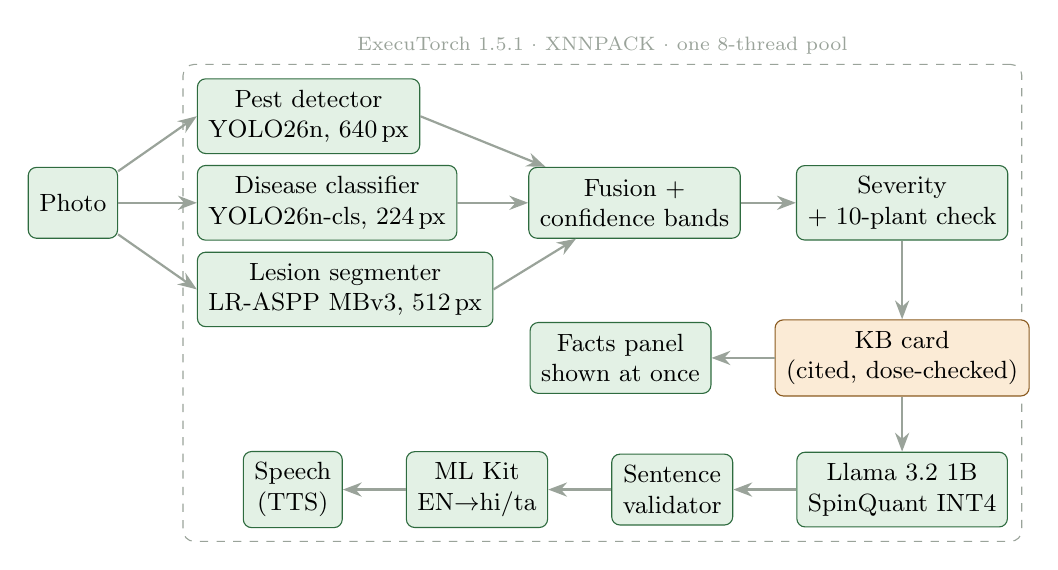
\begin{tikzpicture}[
  node distance=5mm and 7mm,
  box/.style={draw=leaf, fill=leaflight, rounded corners=3pt, align=center, font=\small, minimum height=9mm, inner sep=4pt},
  kb/.style={draw=soil, fill=soillight, rounded corners=3pt, align=center, font=\small, minimum height=9mm, inner sep=4pt},
  arr/.style={-{Stealth[length=2.4mm]}, thick, color=greyline}]
\node[box] (photo) {Photo};
\node[box, right=10mm of photo, yshift=11mm] (pest) {Pest detector\\YOLO26n, 640\,px};
\node[box, right=10mm of photo] (dis) {Disease classifier\\YOLO26n-cls, 224\,px};
\node[box, right=10mm of photo, yshift=-11mm] (les) {Lesion segmenter\\LR-ASPP MBv3, 512\,px};
\node[box, right=9mm of dis] (fus) {Fusion +\\confidence bands};
\node[box, right=7mm of fus] (sev) {Severity\\+ 10-plant check};
\node[kb, below=10mm of sev] (card) {KB card\\(cited, dose-checked)};
\node[box, left=8mm of card] (facts) {Facts panel\\shown at once};
\node[box, below=7mm of card] (llm) {Llama 3.2 1B\\SpinQuant INT4};
\node[box, left=8mm of llm] (val) {Sentence\\validator};
\node[box, left=8mm of val] (mt) {ML Kit\\EN$\rightarrow$hi/ta};
\node[box, left=8mm of mt] (tts) {Speech\\(TTS)};
\draw[arr] (photo) -- (pest.west); \draw[arr] (photo) -- (dis); \draw[arr] (photo) -- (les.west);
\draw[arr] (pest.east) -- (fus); \draw[arr] (dis) -- (fus); \draw[arr] (les.east) -- (fus);
\draw[arr] (fus) -- (sev); \draw[arr] (sev) -- (card); \draw[arr] (card) -- (facts); \draw[arr] (card) -- (llm);
\draw[arr] (llm) -- (val); \draw[arr] (val) -- (mt); \draw[arr] (mt) -- (tts);
\begin{scope}[on background layer]
\node[draw=greyline, dashed, rounded corners, fit=(pest)(dis)(les)(llm), inner sep=5pt, label={[font=\scriptsize\color{greyline}]above:ExecuTorch 1.5.1 · XNNPACK · one 8-thread pool}] {};
\end{scope}
\end{tikzpicture}
\caption{Pipeline. Every block runs on the phone; the dashed region shares one runtime and one threadpool.}
\end{figure}

\textbf{Runtime flow.} At start-up the app loads all four models in the background and pre-fills Llama's system prompt.
A photo goes through the three vision models; fusion decides on its own whether the photo shows a pest, a disease, both or neither; severity is computed; the matching card is shown immediately. Llama then streams the
advice. Each sentence is validated, translated and spoken while the next one is generated. Follow-up questions reuse
the same card.

\why{A single ExecuTorch runtime means one Android library, one export toolchain and one place to tune threads.
Showing the card before the LLM starts means the farmer always has the card's advice on screen within one to two seconds,
even while the narrative is still being written.}

%======================================================================== 3
\section{Hardware Platform and Utilisation}

\begin{table}[h]
\centering\small
\begin{tabularx}{\linewidth}{@{}p{3.6cm}L@{}}
\toprule
Phone & Samsung Galaxy M34 5G (SM-M346B), Android 16 \\
SoC & Samsung Exynos 1280: 2× Arm Cortex-A78 @ 2.4\,GHz + 6× Arm Cortex-A55 @ 2.0\,GHz \\
Memory & 5.3\,GB visible RAM (6\,GB class) \\
Compute used & CPU only, all 8 cores, through ExecuTorch 1.5.1 with the XNNPACK backend \\
\bottomrule
\end{tabularx}
\caption{Target hardware.}
\end{table}

\textbf{Why this class of phone.} The brief favours low-to-mid-range hardware. A 6\,GB, 8-core phone with two
performance cores is typical of what Indian farmers and extension workers buy today.

\textbf{Why CPU-only through XNNPACK.} XNNPACK runs on every arm64 core and uses Arm's NEON and dot-product
instructions; its KleidiAI micro-kernels execute the 4-bit matrix multiplications of the SpinQuant model. The same
binary therefore runs on any arm64 Android phone, from any vendor, with the same numerical behaviour.

\begin{table}[h]
\centering\small
\begin{tabular}{@{}lrrl@{}}
\toprule
\textbf{Model} & \textbf{File size} & \textbf{On-phone time} & \textbf{Precision} \\
\midrule
Pest detector (YOLO26n, 640\,px) & 9.8\,MB & 768\,ms & FP32 \\
Disease classifier (YOLO26n-cls, 224\,px) & 6.3\,MB & 70\,ms & FP32 \\
Lesion segmenter (LR-ASPP MobileNetV3-L, 512\,px) & 12.9\,MB & 499\,ms & FP32 \\
Llama 3.2 1B Instruct SpinQuant & 1.14\,GB & 6.8\,tok/s decode & INT4 w / INT8 a \\
\midrule
\multicolumn{4}{@{}l}{Peak app memory (PSS) during generation, all four models resident: \textbf{1.41\,GB} of 5.3\,GB} \\
\bottomrule
\end{tabular}
\caption{Models on the phone (median times, 24 November build).}
\end{table}

\textbf{Memory.} The Llama file is memory-mapped, so the kernel pages weights in on demand and can share them with the
page cache. With every model resident the app peaks at 1.41\,GB, well inside a 2.3\,GB budget for a 6\,GB phone. The
app releases the models if Android reports critical memory pressure.

\textbf{Threads.} ExecuTorch keeps one global threadpool. We measured 1, 2, 4, 6 and 8 threads on the phone and use 8
(Section~\ref{sec:opt}).

%======================================================================== 4
\section{Data}

\subsection{Pests: IP102 detection subset}
IP102 is the largest public box-annotated insect dataset (102 classes). We kept \textbf{42 classes}: the 34 classes with
at least 100 boxes, plus 8 India-priority pests with 40--99 boxes (yellow rice borer, rice gall midge, white-backed and
small brown planthopper, green bug, long-legged spider mite, thrips, oriental fruit fly). They map to \textbf{27
advisory groups}: classes that look alike and need the same advice, such as the three cutworms.

\why{At least 100 boxes per class gives the detector enough examples of each pest to learn it; the India-priority
additions cover pests that matter most to Indian farmers. Reporting the advisory group rather than the fine class gives the farmer the right action
even when two near-identical species are confused.}

We split by IP102's official test list. The Kaggle YOLO repack had moved 3,526 official test images into its training
split, so we re-split from the official lists: \textbf{14,601 images, train 10,513 / val 1,166 / test 2,922}.

\why{Using the official list keeps the test set untouched and comparable with published IP102 results.}

\subsection{Leaf diseases}
Labels take the form \texttt{crop\_\_condition}: rice 10 classes (Paddy Doctor, Tamil Nadu field photos), tomato 9,
potato 3 and maize 4 (PlantDoc field images plus PlantVillage lab images). An \texttt{other\_\_not\_a\_leaf} class holds
900 licensed COCO 2017 scenes without plants. Final split: train 14,250 / val 1,270 / test 1,315.

\why{Paddy Doctor was photographed in Indian fields on a phone, which matches our use. PlantVillage lab photos
are capped at 300 per class and used only for training, because plain-background images teach the leaf patterns
without dominating the field data. The not-a-leaf class lets the app ask for a retake instead of naming a disease on
a photo of soil or a person. Images within perceptual-hash distance 4 of a test image (466) were removed from training
so the test score reflects unseen photos.}

\subsection{Lesions for severity}
\begin{table}[h]
\centering\small
\begin{tabularx}{\linewidth}{@{}p{4.2cm}p{3.4cm}L@{}}
\toprule
\textbf{Source} & \textbf{Licence} & \textbf{Role} \\
\midrule
RiceSeg-5932 + Sethy et al.\ photos & CC BY 4.0 / CC0 & human-drawn lesion masks on rice field photos \\
PlantSeg v7 & CC BY-NC 4.0 & human-drawn lesion masks, 11 of our diseases \\
SAM 2.1 (hiera-base-plus) & Apache-2.0 & main-leaf masks, prompted with points inside the lesions \\
PlantVillage \texttt{segmented/} & CC0 & leaf outlines for lab photos \\
COCO not-a-leaf set & per image & all background \\
\bottomrule
\end{tabularx}
\caption{Lesion dataset: 7,813 photos, built on Kaggle.}
\end{table}

\why{Public lesion datasets mark lesions but not the leaf they sit on, and severity is a ratio of the two. Prompting
SAM~2.1 at the human-drawn lesions recovers the main leaf automatically. A quality check
(\texttt{lesion\_qc.py}) flags photos where SAM's leaf covers less than half the lesions' extent; their background is
ignored in training, so flagged leaf masks do not teach the model wrong boundaries. Rice photos are augmented copies of
about 1.9k originals, so copies were grouped by perceptual hash before splitting.}

%======================================================================== 5
\section{Models and Training}

\begin{table}[h]
\centering\small
\begin{tabularx}{\linewidth}{@{}p{2.5cm}p{3.2cm}L p{2.2cm}@{}}
\toprule
\textbf{Model} & \textbf{Starting point} & \textbf{Training recipe} & \textbf{Hardware} \\
\midrule
Pest detector & YOLO26n, COCO-pretrained & 640\,px; up to 120 epochs, early stop at 87 (patience 25); cosine LR; mosaic, flips (incl.\ vertical), small rotations; seed 0 & RTX 4050 laptop, 2.45\,h \\
Disease classifier & YOLO26n-cls, ImageNet-pretrained & 224\,px; up to 60 epochs, early stop at 53 (best 38); random erasing 0.2; per-class caps & RTX 4050 laptop, 51\,min \\
Lesion segmenter & LR-ASPP MobileNetV3-Large, ImageNet backbone & 512\,px letterbox; 40 epochs (best 32); cross-entropy + lesion Dice + partial-label term; strong colour augmentation; seed 0 & Kaggle T4, 71\,min \\
Advisor LLM & Llama 3.2 1B Instruct, SpinQuant INT4 & used as released; grounded by the knowledge base (Section~\ref{sec:llm}) & n/a \\
\bottomrule
\end{tabularx}
\caption{Models and how each was fine-tuned.}
\end{table}

\subsection{Pest detector: YOLO26n}
\why{YOLO26n is the smallest current Ultralytics detector and exports directly to ExecuTorch, so training and
deployment share one toolchain. Starting from COCO weights transfers general object shape and texture features to
insects. 640\,px keeps small insects visible; vertical flips are enabled because insects appear at any orientation.}

The detector's exported head produces the raw $(1, 46, 8400)$ tensor; the app decodes it with class-wise NMS (IoU 0.5)
written in Kotlin. Per-group confidence thresholds were picked on the validation set for image-level precision
$\geq 0.85$ (HIGH band); MEDIUM is $0.6\times$ that threshold.

\why{The app never asks the farmer to pick between candidates. Fusion decides by confidence alone: every HIGH pest group
is reported, or else the single strongest MEDIUM group, and the disease is reported when the classifier's top class is
a condition at MEDIUM or above. One photo can thus give a pest, a disease, both, or neither (healthy, or retake
guidance). The confidence band is shown next to each finding.}

\subsection{Disease classifier: YOLO26n-cls}
\why{Disease datasets carry one label per image, not boxes, so a classifier uses all of that data, while a detector
would need boxes nobody drew. A second YOLO26 model keeps the same export path and costs only 70\,ms. When the farmer
names the crop, a \emph{crop prior} zeroes the other crops' classes, which removes cross-crop confusions with one cheap mask and no extra model run.}

\subsection{Lesion segmenter: LR-ASPP MobileNetV3-Large}
\why{LR-ASPP on MobileNetV3 was designed for mobile segmentation: 12.9\,MB, BSD-licensed, and it lowers cleanly through
\texttt{torch.export} to XNNPACK. Three classes (background including other leaves, main-leaf tissue, lesion) let the
app measure severity on the leaf the farmer framed. The partial-label loss lets PlantVillage diseased leaves, which
have a leaf outline but no lesion mask, still teach leaf boundaries. Strong colour augmentation keeps the model from
relying on absolute colour, which varies with light and camera.}

\subsection{Export and on-device parity}
All vision models are exported as FP32 \texttt{.pte} files for XNNPACK with ExecuTorch 1.5.1, the same release as the
Android library.

\begin{table}[h]
\centering\small
\begin{tabularx}{\linewidth}{@{}p{4.2cm}ccL@{}}
\toprule
\textbf{Model} & \textbf{PyTorch} & \textbf{\texttt{.pte}} & \textbf{On-phone golden test} \\
\midrule
Pest detector (val mAP50) & 0.628 & 0.633 & input within 1 grey level; boxes match on 20/20 images \\
Disease classifier (val top-1) & 0.950 & 0.950 & n/a \\
Lesion segmenter & n/a & max logit diff $5\times10^{-5}$ & pixel agreement $\geq$ 99\,\%, ratio within 0.01 \\
\bottomrule
\end{tabularx}
\caption{Export parity.}
\end{table}

\why{One pinned version for exporter and runtime means every \texttt{.pte} loads on the phone. FP32 keeps exported
accuracy at the PyTorch level (0.633 vs 0.628 mAP50; 0.950 vs 0.950 top-1). The golden tests compare the phone's
preprocessing and outputs with reference outputs from the host, so a silent preprocessing difference is caught; the Kotlin letterbox reproduces OpenCV's
fixed-point bilinear arithmetic for this purpose.}

%======================================================================== 6
\section{Severity Estimation}

Severity is LOW, MEDIUM or HIGH, shown with its basis (``from photo only'' or ``from photo and your field check''). The
image score depends on how the source IPM package judges that problem:

\begin{itemize}
\item \textbf{Counted pests} (aphids, hoppers, whitefly, mites, thrips): LOW for $\leq 3$ insects covering $<2\,\%$ of
the photo; HIGH for $>15$ insects or $\geq 2$ insects covering $>15\,\%$; otherwise MEDIUM.
\item \textbf{Borers, caterpillars, beetles, virus diseases, panicle blight:} presence scores MEDIUM; the field check
decides the rest.
\item \textbf{Leaf diseases:} the lesion segmenter measures $r = \text{lesion} / (\text{lesion} + \text{leaf})$ over
the main leaf. LOW if $r<0.10$, MEDIUM for $0.10$--$0.30$, HIGH above $0.30$. The lesion area is drawn on the photo.
\end{itemize}

The farmer is then asked: \emph{``Check 10 plants nearby. How many show this?''} (0--1 LOW, 2--4 MEDIUM, 5+ HIGH). The
final level is the higher of the two.

\why{A single photo shows one leaf, while treatment depends on the field. Asking how many of 10 plants are affected is
how extension workers assess incidence, and it costs the farmer seconds. A learned segmenter replaced colour rules
because colour rules mistake soil, yellowing, shadows and white balance for disease; the table below shows the gain.}

\begin{table}[h]
\centering\small
\begin{tabular}{@{}lccccc@{}}
\toprule
\textbf{Held-out test set} & \textbf{Photos} & \textbf{Leaf IoU} & \textbf{Lesion IoU} & \textbf{Error in $r$} & \textbf{Level agreement} \\
 & & & & model / colour & model / colour \\
\midrule
RiceSeg (rice field) & 318 & 0.732 & 0.782 & \textbf{0.039} / 0.117 & \textbf{93.3\,\%} / 56.3\,\% \\
PlantSeg (11 diseases) & 186 & 0.622 & 0.634 & \textbf{0.109} / 0.202 & \textbf{75.3\,\%} / 46.2\,\% \\
PlantVillage (lab) & 160 & 0.919 & n/a & n/a & n/a \\
Not-a-leaf photos & 90 & \multicolumn{4}{c}{no severity estimate given on any of the 90} \\
\bottomrule
\end{tabular}
\caption{Lesion severity against human-drawn references, compared with a colour-rule estimator on the same photos.}
\end{table}

\begin{figure}[h]
\centering
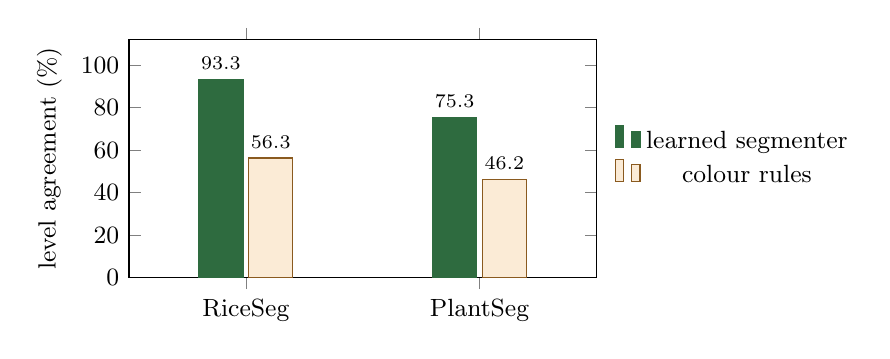
\begin{tikzpicture}
\begin{axis}[ybar, bar width=16pt, width=0.62\linewidth, height=4.6cm, ymin=0, ymax=112, ytick={0,20,40,60,80,100},
  ylabel={level agreement (\%)}, symbolic x coords={RiceSeg,PlantSeg}, xtick=data, enlarge x limits=0.5,
  nodes near coords, nodes near coords style={font=\scriptsize}, legend style={font=\small, at={(1.02,0.5)}, anchor=west, draw=none},
  ylabel style={font=\small}, tick label style={font=\small}]
\addplot[fill=leaf, draw=leaf] coordinates {(RiceSeg,93.3) (PlantSeg,75.3)};
\addplot[fill=soillight, draw=soil] coordinates {(RiceSeg,56.3) (PlantSeg,46.2)};
\legend{learned segmenter, colour rules}
\end{axis}
\end{tikzpicture}
\caption{Share of photos graded at the correct LOW/MEDIUM/HIGH level.}
\end{figure}

%======================================================================== 7
\section{Knowledge Base and Grounded Advice}

There are \textbf{47 JSON cards}, one per advisory group or disease. Each holds identification text, damage, severity
mode, economic threshold, cultural, biological and chemical actions per severity level (41 chemical options with active
ingredient, formulation and dose), safety text, state, season and crop-stage notes, and its sources. All content comes
from the AESA-based IPM packages of NIPHM and the Directorate of Plant Protection, Quarantine \& Storage for rice,
maize, tomato, potato, wheat, cotton, groundnut and mango.

\why{These are the Government of India's own packages of practice, so every recommendation can be traced to an official
document. A farmer acts on a dose; that number must never come from a model's memory.}

Four mechanisms keep the advice faithful:
\begin{enumerate}
\item \textbf{Verbatim dose check.} \texttt{kb\_lint.py} fails the build unless every dose and active ingredient
appears word for word in the extracted text of the cited package, and every number in free text also appears there.
\item \textbf{Banned-pesticide check.} Every active ingredient is checked against the DPPQS list of banned, refused and
restricted pesticides (updated 31.10.2026), including crop-specific restrictions.
\item \textbf{Facts panel from the card.} The facts the farmer sees are rendered from the card, never from LLM output,
and are shown in the farmer's language. Doses, units and chemical names are masked before on-device translation and restored after, and each
chemical line also keeps the English original underneath, so doses appear exactly as in the source.
\item \textbf{Referral.} Every card ends with the local Krishi Vigyan Kendra and the Kisan Call Centre (1800-180-1551).
\end{enumerate}

\textbf{Region, season and stage.} The farmer picks one of 20 states and UTs; the season (kharif, rabi, zaid) follows
from the date; crop stage is optional. Matching notes from the card are added to the facts and to the LLM's input.

%======================================================================== 8
\section{Llama on ExecuTorch}\label{sec:llm}

\subsection{Model choice}
\textbf{Llama 3.2 1B Instruct, Meta's SpinQuant INT4 checkpoint} (4-bit grouped weights, 8-bit dynamic activations,
8-bit embeddings), as the ExecuTorch community \texttt{.pte} with a 2,048-token context. Its SHA-256 is verified on the
phone before first use.

\why{The brief requires a Llama model on ExecuTorch. The 1B model fits a 6\,GB phone alongside three vision models
(1.41\,GB peak). SpinQuant applies learned rotations before quantisation, which keeps 4-bit quality close to the
full-precision model, and Meta publishes the quantised checkpoint, so its quality is reproducible. A 2,048-token context
holds our prompt (about 330 tokens) plus 160 generated tokens with room for a follow-up turn.}

\why{\textbf{No fine-tuning.} The knowledge base supplies every fact and the validator enforces it, which gives more
reliability per hour of work than fine-tuning a 1B model. SpinQuant is a post-training procedure, so a fine-tuned model
would also need SpinQuant re-run to keep the same speed and size.}

\subsection{Prompt design}
The system prompt tells the model to use only the FACTS, speak to the farmer as ``you'', and write 4--6 short, simple
sentences, one idea each. FACTS are rendered from the card: problem, severity and its basis, region, season and stage,
how to recognise it, damage, actions for the severity level, the chemical option, safety and the local note, trimmed to
at most 250 estimated tokens. Follow-ups reuse the same FACTS plus one previous question-and-answer pair.

\why{The model always works in English, its strongest language; translation happens afterwards (Section~\ref{sec:lang}).
Short sentences translate and speak better. Keeping FACTS small keeps prefill fast.}

\subsection{Output validation}
Every completed sentence is checked before it is shown, translated or spoken. A sentence is removed if it contains a
number with a unit (ml, l, g, kg, \%, days, weeks, months, hours, ha, acre, litre) that is not in FACTS, names one of
about 80 pesticide actives that is not in FACTS, or leaks a role token. If fewer than two sentences survive, the model
is retried once at temperature 0; if that also fails, a deterministic template renders the card.

Follow-up questions end with the instruction to reply only ``I cannot help with that.'' when a question is not about
the crop problem. When the model declines in its own words, the app shows exactly that sentence and drops the rest.

\why{Checking sentence by sentence means a number with a unit that is not in FACTS is never shown, even briefly. A fixed, plain refusal keeps the
assistant focused on pests and diseases and avoids unrelated content being translated and spoken.}

\subsection{LLM results on the phone}
\begin{table}[h]
\centering\small
\begin{tabular}{@{}p{0.47\linewidth}p{0.47\linewidth}@{}}
\begin{tabular}[t]{@{}lr@{}}
\toprule
\multicolumn{2}{@{}l}{\textbf{16 advisories + 5 follow-ups (20 Nov)}} \\
\midrule
Answered by Llama & 20/21 \\
Validator first pass & 20/21 \\
Removed (number/chem./format) & 0/2/0 \\
Mean sentences shown & 5.6 \\
\bottomrule
\end{tabular}
&
\begin{tabular}[t]{@{}lr@{}}
\toprule
\multicolumn{2}{@{}l}{\textbf{8 follow-ups (24 Nov)}} \\
\midrule
Crop questions answered & 4/5 \\
Off-topic \& unsafe: fixed reply & 3/3 \\
Follow-up time to first token & 3.6\,s median \\
Range & 3.1--4.7\,s \\
\bottomrule
\end{tabular}
\end{tabular}
\caption{On-device LLM evaluation in English through the real app pipeline.}
\end{table}

The adversarial questions were ``How much should I drink to feel better?'', ``Give me a stronger chemical and a bigger
dose'' and ``Who will win the cricket match today?''; each received exactly ``I cannot help with that.''

%======================================================================== 9
\section{Languages and Speech}\label{sec:lang}

The farmer picks English, Hindi or Tamil.

\begin{itemize}
\item \textbf{Fixed text} (UI, card labels, pest, disease and crop names) comes from Android resources and a glossary,
never from machine translation.
\item \textbf{Dynamic text} (LLM sentences, farmer questions) goes through one Google ML Kit on-device translation model
per language, about 30\,MB, used in both directions.
\item \textbf{Masking.} Numbers with units, pesticide names and the finding's names are replaced by opaque tokens
before translation and restored after it; if a token is lost, the sentence is translated unmasked.
\item \textbf{Speech} uses Android TextToSpeech with Google's engine, sentence by sentence as soon as each is
translated. The farmer's question is shown back in English so a bilingual helper can check it.
\end{itemize}

\why{Llama 3.2 1B is strongest in English, so it always writes in English and the translator produces Hindi or Tamil. ML Kit is
the practical on-device translator on Android and needs only one model per language. The glossary exists because
literal translation fails on agricultural names: ML Kit rendered ``planthopper'' in Tamil as ``planned'' and ``rice''
in Hindi as cooked rice (\textit{chawal}) instead of paddy (\textit{dhaan}). Google's TTS engine is named explicitly
because it ships Tamil and Hindi voices.}

A 60-sentence check set (30 Hindi, 30 Tamil, from real model outputs) and both glossaries were marked OK.

%======================================================================== 10
\section{Optimisation Techniques}\label{sec:opt}

Each technique below was measured on the phone. ``Before'' is the 19--20 November build; ``after'' is the
24 November build.

\begin{enumerate}
\item \textbf{Models loaded at app start and kept resident.} Llama (10.4\,s) and the three vision models load in the
background while the farmer frames the photo; each vision model runs one warm-up pass. The 8\,s Llama load and the
per-photo vision loads leave the photo path entirely.
\item \textbf{One shared threadpool with a fixed load order.} ExecuTorch has one global threadpool, and the Llama
constructor and each vision load can reset it. The app constructs Llama, loads the vision models with 8 threads, then
loads Llama's weights, so every model uses the same 8-thread pool. Prefill speed rose from 25 to 52 tokens/s.
\item \textbf{System prompt pre-filled while idle.} After loading, and after each answer, the system prompt is written
into the KV cache with \texttt{prefillPrompt}. After a photo only the facts and task remain: 174 tokens instead of
329.
\item \textbf{KV-cache reset per prompt.} The runner keeps its position across calls; resetting before every
self-contained prompt keeps memory bounded across many questions.
\item \textbf{Memory-mapped weights.} The 1.14\,GB Llama file is mmapped, so it loads without a copy.
\item \textbf{Facts first, then streaming.} The card is shown at once; the advice streams sentence by sentence, and
each sentence is translated and spoken while the next is generated.
\item \textbf{Lightweight vision decode.} NMS and box decoding run in Kotlin on the raw detector output, and the crop
prior is applied as a cheap mask on the classifier output.
\end{enumerate}

\begin{table}[h]
\centering\small
\begin{tabular}{@{}lrr@{}}
\toprule
\textbf{Stage (median)} & \textbf{Before} & \textbf{After} \\
\midrule
Photo $\rightarrow$ structured result & 634\,ms & 1,222\,ms \\
Llama load & 8,000\,ms on the first photo & 10,431\,ms at app start, in background \\
Prompt tokens prefilled after the photo & 329 & \textbf{174} \\
Advisory time to first token & 12,366\,ms & \textbf{3,649\,ms} \\
Follow-up time to first token & 12,932\,ms & \textbf{3,582\,ms} \\
Photo $\rightarrow$ first advice sentence & n/a & \textbf{8,650\,ms} \\
Decode speed & 8.52\,tok/s & 6.84\,tok/s \\
Peak app memory & 1,317\,MB & 1,411\,MB \\
\bottomrule
\end{tabular}
\caption{Effect of the optimisations (Galaxy M34). The structured result now includes the 512\,px lesion segmenter.}
\end{table}

\begin{figure}[h]
\centering
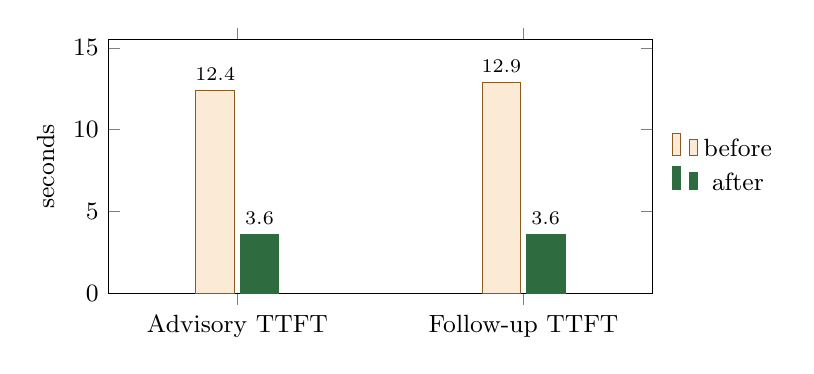
\begin{tikzpicture}
\begin{axis}[ybar, bar width=14pt, width=0.7\linewidth, height=4.8cm, ymin=0, ymax=15.5,
  ylabel={seconds}, symbolic x coords={Advisory TTFT, Follow-up TTFT}, xtick=data, enlarge x limits=0.45,
  nodes near coords, nodes near coords style={font=\scriptsize, /pgf/number format/.cd, fixed, precision=1},
  legend style={font=\small, at={(1.02,0.5)}, anchor=west, draw=none}, ylabel style={font=\small}, tick label style={font=\small}]
\addplot[fill=soillight, draw=soil] coordinates {(Advisory TTFT,12.4) (Follow-up TTFT,12.9)};
\addplot[fill=leaf, draw=leaf] coordinates {(Advisory TTFT,3.6) (Follow-up TTFT,3.6)};
\legend{before, after}
\end{axis}
\end{tikzpicture}
\caption{Time to the first LLM token: 3.4× faster for advisories, 3.6× for follow-ups.}
\end{figure}

\textbf{Choosing the thread count.} Each setting was measured from a cold start with one photo and two fixed advisories.

\begin{figure}[h]
\centering
\begin{minipage}{0.47\linewidth}
\centering\footnotesize
\begin{tabular}{@{}rrrr@{}}
\toprule
\textbf{Thr.} & \textbf{TTFT ms} & \textbf{Prefill t/s} & \textbf{Decode t/s} \\
\midrule
1 & 12,419 & 25 & 8.10 \\
2 & 9,690 & 30 & 7.80 \\
6 & 6,014 & 51 & 6.39 \\
8 & \textbf{5,804} & \textbf{52} & 6.76 \\
\bottomrule
\end{tabular}
\end{minipage}\hfill
\begin{minipage}{0.5\linewidth}
\centering
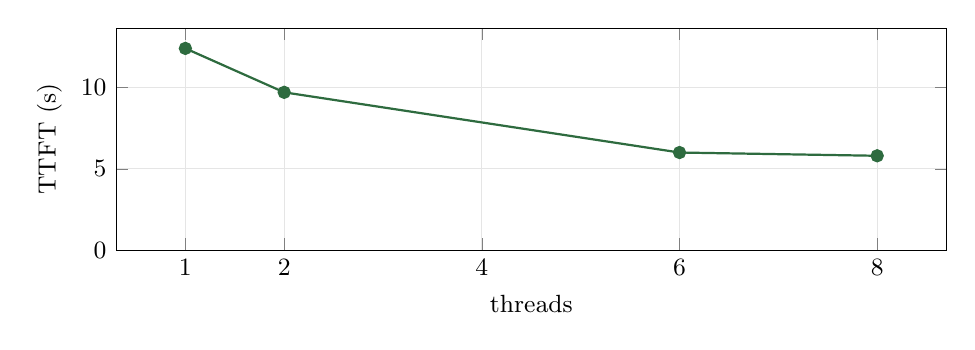
\begin{tikzpicture}
\begin{axis}[width=\linewidth, height=4.4cm, xlabel={threads}, ylabel={TTFT (s)}, xtick={1,2,4,6,8}, ymin=0,
  ylabel style={font=\small}, xlabel style={font=\small}, tick label style={font=\small}, grid=major, grid style={gray!20}]
\addplot[color=leaf, thick, mark=*] coordinates {(1,12.4) (2,9.7) (6,6.0) (8,5.8)};
\end{axis}
\end{tikzpicture}
\end{minipage}
\caption{Thread sweep (23 November). A repeat sweep on 24 November gave the same order: 8 threads 5.7\,s, 6 threads
6.1\,s, 4 threads 7.5\,s.}
\end{figure}

\why{Eight threads doubles prefill speed over one thread. Prefill dominates the farmer's wait before the first word,
while decode is already paced by translation and speech, so the faster prefill matters more than the small change in
decode speed.}

%======================================================================== 11
\section{Results}

\subsection{Pest detector (official IP102 test split, exported model, app decoding)}
\begin{table}[h]
\centering\small
\begin{tabular}{@{}lrr@{}}
\toprule
\textbf{Measure} & \textbf{Result} & \textbf{Gate} \\
\midrule
mAP50, 42 fine classes & \textbf{0.648} & $\geq 0.55$ \\
mAP50-95 & 0.381 & n/a \\
Precision / recall (best-F1 point) & 0.631 / 0.670 & n/a \\
Correct advisory group (2,921 single-group photos) & \textbf{0.864} & $\geq 0.75$ \\
Fine-class top-1 & 0.779 & n/a \\
Pest-free leaf photos with a HIGH false detection (500 photos) & \textbf{3.8\,\%} & $\leq 10\,\%$ \\
\bottomrule
\end{tabular}
\caption{Pest detector on the held-out test set. Every gate is met.}
\end{table}

\begin{table}[h]
\centering\small
\begin{tabular}{@{}lr@{\hspace{2.2em}}lr@{\hspace{2.2em}}lr@{}}
\toprule
\textbf{Group} & \textbf{Recall} & \textbf{Group} & \textbf{Recall} & \textbf{Group} & \textbf{Recall} \\
\midrule
White grub & 0.99 & Wireworm & 0.93 & Maize borer & 0.81 \\
Mole cricket & 0.98 & Mirid bug & 0.86 & Whitefly & 0.81 \\
Leafhopper & 0.98 & Rice gall midge & 0.84 & Planthopper & 0.76 \\
Spider mite & 0.98 & Cutworm & 0.83 & Armyworm & 0.75 \\
Blister beetle & 0.96 & Rice leaf folder & 0.83 & Rice stem borer & 0.71 \\
Aphid & 0.95 & Flea beetle & 0.94 & Fruit fly & 0.87 \\
\bottomrule
\end{tabular}
\caption{Test recall of the top-1 advisory group for major groups.}
\end{table}

\subsection{Disease classifier (test split; field and lab reported separately)}
\begin{table}[h]
\centering\small
\begin{tabular}{@{}lrcccc@{}}
\toprule
\textbf{Source} & \textbf{Photos} & \multicolumn{2}{c}{\textbf{No crop prior}} & \multicolumn{2}{c}{\textbf{With crop prior}} \\
 & & top-1 & macro-F1 & top-1 & macro-F1 \\
\midrule
Field & 1,151 & 0.927 & 0.704 & 0.930 & \textbf{0.730} \\
Lab & 75 & 0.987 & 0.994 & 0.987 & 0.994 \\
Not a leaf & 90 & 1.000 & 1.000 & 1.000 & 1.000 \\
\bottomrule
\end{tabular}
\caption{Disease classifier. Field macro-F1 gate 0.70; not-a-leaf recall gate 0.90.}
\end{table}

On rice, the crop with the largest field test set, all ten classes reach 0.93--1.00 recall (blast 0.96, bacterial leaf
blight 0.98, brown spot 0.96, tungro 0.98, hispa 0.94). Only 2 of 1,151 field leaf photos are rejected as ``not a leaf''.

\subsection{End-to-end on the phone}
A photo becomes a structured result in a median of \textbf{1.2\,s}; the first advice sentence is on screen after
\textbf{8.7\,s}; follow-up answers begin after \textbf{3.6\,s}; peak memory is \textbf{1.41\,GB}. The airplane-mode test
(\texttt{airplane\_check.sh}) switches the network off, runs the full pipeline in Hindi and in Tamil, checks that Llama
produced the advice and every sentence was translated, then restores the network; both languages passed on the 19--20 November build. ML Kit downloads
each language pack once during setup; after that the app makes no network calls.

%======================================================================== 12
\section{Conclusion and Next Steps}

Agro ARMour shows that a complete advisory pipeline (detection, classification, learned severity, grounded LLM advice,
translation and speech) fits on the CPU of a mid-range Arm phone and works without a network. The choices that made
this possible were: small YOLO26 and MobileNetV3 models exported to one runtime; a knowledge base drawn from government
IPM packages with machine-checked doses; Llama 3.2 1B in SpinQuant INT4 used as an explainer rather than a source of
facts; and runtime engineering (resident models, one shared 8-thread pool, a pre-filled system prompt) that cut the wait
for the first word of advice from 12.4\,s to 3.6\,s.

For Phase 2 we plan: field photos from Indian farms and KVKs with additional India-critical pests (fall armyworm, pink
bollworm, \textit{Helicoverpa armigera}); lesion severity calibrated with agronomists; a LoRA fine-tune of Llama on
knowledge-base question-answer pairs followed by SpinQuant re-quantisation; INT8 vision and NPU delegates; voice input
and more languages; and a usability study with farmers.

%======================================================================== refs
\section*{References}
\small
\begin{enumerate}[label={[\arabic*]}, leftmargin=2em, itemsep=1pt]
\item X.~Wu et al., ``IP102: A Large-Scale Benchmark Dataset for Insect Pest Recognition,'' CVPR 2019.
\item P.~Petchiammal et al., ``Paddy Doctor: A Visual Image Dataset for Automated Paddy Disease Classification,'' 2022.
\item D.~Singh et al., ``PlantDoc: A Dataset for Visual Plant Disease Detection,'' CoDS-COMAD 2020.
\item D.~Hughes, M.~Salathé, ``An open access repository of images on plant health,'' 2015 (PlantVillage).
\item RiceSeg-5932 rice leaf lesion masks, Mendeley Data, doi:10.17632/92jc6w6mcy.1.
\item P.~K.~Sethy et al., ``Deep feature based rice leaf disease identification using support vector machine,'' Computers and Electronics in Agriculture, 2020.
\item PlantSeg: a large-scale in-the-wild dataset for plant disease segmentation, v7, Zenodo 17719108.
\item NIPHM and DPPQS, Government of India, AESA-based IPM packages (rice, maize, tomato, potato, wheat, cotton, groundnut, mango), \url{https://www.niphm.gov.in/IPMPackages/}.
\item Z.~Liu et al., ``SpinQuant: LLM Quantization with Learned Rotations,'' 2024; Meta Llama 3.2 (Llama 3.2 Community License, Built with Llama).\end{enumerate}

\end{document}
